% DO NOT COMPILE THIS FILE DIRECTLY!
% This is included by the other .tex files.

\colorlet{punct}{red!60!black}
\definecolor{background}{HTML}{EEEEEE}
\definecolor{delim}{RGB}{20,105,176}
\colorlet{numb}{magenta!60!black}

\lstdefinelanguage{json}{
    basicstyle=\ttfamily\footnotesize,
    numbers=left,
    numberstyle=\ttfamily\footnotesize,
    stepnumber=1,
    numbersep=8pt,
    showstringspaces=false,
    breaklines=true,
    frame=lines,
    backgroundcolor=\color{background},
    literate=
     *{0}{{{\color{numb}0}}}{1}
      {1}{{{\color{numb}1}}}{1}
      {2}{{{\color{numb}2}}}{1}
      {3}{{{\color{numb}3}}}{1}
      {4}{{{\color{numb}4}}}{1}
      {5}{{{\color{numb}5}}}{1}
      {6}{{{\color{numb}6}}}{1}
      {7}{{{\color{numb}7}}}{1}
      {8}{{{\color{numb}8}}}{1}
      {9}{{{\color{numb}9}}}{1}
      {:}{{{\color{punct}{:}}}}{1}
      {,}{{{\color{punct}{,}}}}{1}
      {\{}{{{\color{delim}{\{}}}}{1}
      {\}}{{{\color{delim}{\}}}}}{1}
      {[}{{{\color{delim}{[}}}}{1}
      {]}{{{\color{delim}{]}}}}{1},
}

\begin{frame}[t,plain]
\titlepage
\end{frame}

\begin{frame}
    \frametitle{MISP Feed - Basics}
    MISP Feeds provide a way to
    \begin{itemize}
            \item {\bf Exchange information via any transports} (e.g. HTTP, TLS, USB keys)
        \item Preview events along with their attributes, objects
        \item Select and import events
        \item {\bf Correlate attributes using caching}
    \end{itemize}
     MISP Feeds have the following advantages
        \begin{itemize}
                \item Feeds work without the need of MISP synchronisation (reducing attack surface and complexity to a static directory with the events)\\
    \item {\bf Feeds can be produced without a MISP instance} (e.g. security devices, honeypot sensors)
            \note{Feeds can be used to produce output from various security devices}
        \end{itemize}
\end{frame}

\begin{frame}{Feed - Overview}
        \begin{itemize}
        \item By default, MISP is bundled with $\sim$50 default feeds (MISP feeds, CSV or freetext feeds) which are not enabled by default and described in a simple JSON file\footnote{\url{https://github.com/MISP/MISP/blob/2.4/app/files/feed-metadata/defaults.json}}.
        \item The feeds include CIRCL OSINT feed but also feeds like abuse.ch, Tor exit nodes or many more \footnote{\url{http://www.misp-project.org/feeds/}}.
        \end{itemize}
    \vspace{-25px}
    \begin{figure}
        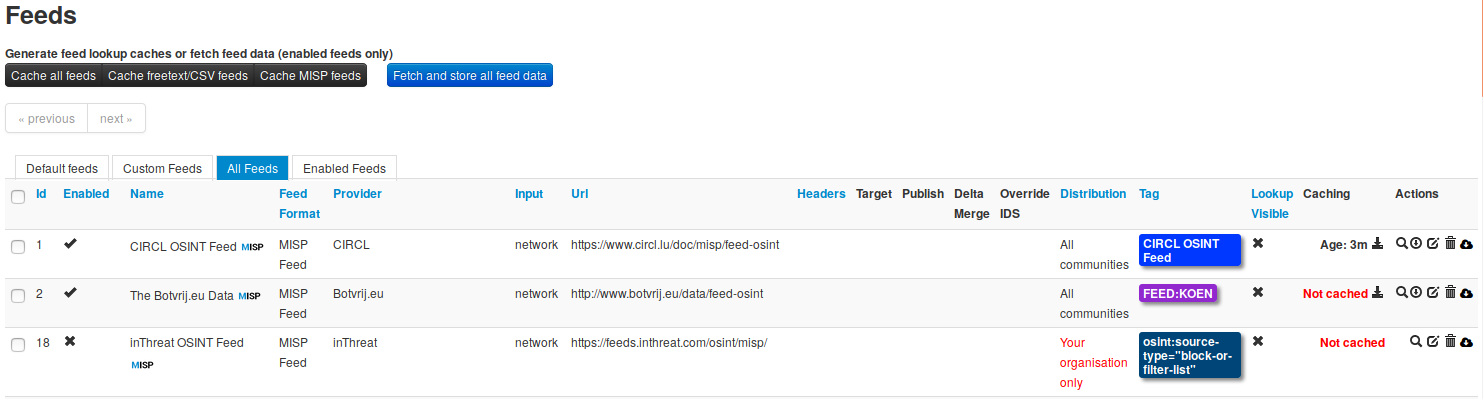
\includegraphics[width=1.05\linewidth]{pics/feeds1.png}
    \end{figure}
\end{frame}

\begin{frame}
    \frametitle{Feed - Operations}
    \begin{figure}
        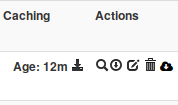
\includegraphics[width=0.35\linewidth]{pics/feeds2.png}
    \end{figure}
    \begin{itemize}
        \item Cache feed attributes for correlation (not imported but visible in MISP)
        \item Disable feed
        \item Explore remote events
        \item Fetch all events (imported in MISP as event)
        \item Edit the feed configuration (e.g. authentication, URL,...)
        \item Remove feed
        \item Download feed metadata (to share feed details)
    \end{itemize}
\end{frame}

\begin{frame}
    \frametitle{Feed - Creation using PyMISP \texttt{feed generator}}
    \texttt{feed generator} fetches events (matching some filtering) from a MISP instance and construct the manifest (defined in \textit{MISP core format}) needed to export data.

    \vspace{15px}
    Particularly,
    \begin{itemize}
        \item Used to generate the {\bf CIRCL OSINT feed}
        \item Export events as json based on tags, organisation, events, ...
        \item Automatically update the dumps and the metadata file
        \item Comparable to a lighweight {\bf TAXII interface}
    \end{itemize}
\end{frame}

\begin{frame}[fragile]
    \frametitle{\texttt{Feed generator} - configuration file}
    \begin{lstlisting}
url = 'your/misp/url'
key = 'YourAPIKey'
ssl = True
outputdir = 'output_directory'

filters = {
    'tag':'tlp:white|feed-export|!privint',
    'org':'CIRCL'
}
# the above would generate a feed for all events created by CIRCL, tagged tlp:white and/or feed-export but exclude anything tagged privint

valid_attribute_distribution_levels = ['0', '1', '2', '3', '4', '5']
# 0: Your Organisation Only
# 4: Sharing Group
# 5: Inherit Event
    \end{lstlisting}
\end{frame}

\begin{frame}
        \frametitle{{\it Real-time} Feed generator - Purpose}
    The PyMISP feed generator is great but may be inadequate or ineficient:
    \begin{itemize}
        \item Batch import of attributes/objects
        \item Data producer doesn't have a MISP instance at hand and only wants to {\bf produce a directly consumable feed}:
    \end{itemize}

    \vspace{15px}
    \begin{center}
        \begin{tikzpicture}[scale=2.0]
        %styles
        \tikzstyle{n}=[ellipse,draw,align=center]
        \tikzstyle{t}=[align=center]
                \tikzstyle{misp}=[rectangle,draw, align=center, fill={rgb:red,0;green,0;blue,3}]
        \tikzstyle{commu}=[->,>=latex,very thick]
        %nodes
        \node[n] (honey) at (0,0) {Honeypot};
                \node[misp] (misp) at (2,0) {\color{white}MISP};
        \node[t] (text) at (1.5,-0.8) {\parbox[l]{3.0cm}{ip-src\\payload-delivery\\url\\malware\\...}};
        %arraws
        \draw[commu] (honey)--(misp);

        \end{tikzpicture}
    \end{center}
\end{frame}

\begin{frame}[fragile]
        \frametitle{{\it Real-time} Feed generator - Usage}
    \begin{itemize}
        \item \texttt{generator.py} exposes a class allowing to generate a MISP feed in real-time
        \item Each items can be appended on daily generated events
    \end{itemize}

    Example:
    \begin{lstlisting}
#  Init generator
generator = FeedGenerator()

#  Adding an attribute to the daily event
attr_type = "ip-src"
attr_value = "8.8.8.8"
additional_data = {}
generator.add_attribute_to_event(attr_type, 
                                 attr_value, 
                                 **additional_data)
\end{lstlisting}
\end{frame}

\begin{frame}[fragile]
        \frametitle{{\it Real-time} Feed generator - Usage (2)}

    \begin{lstlisting}
#  Adding a MISP object (cowrie) to the daily event
obj_name = "cowrie"
obj_data = { 
    "session": "session_id", 
    "username": "admin", 
    "password": "admin", 
    "protocol": "telnet"
    }
generator.add_object_to_event(obj_name, **obj_data)
\end{lstlisting}
\end{frame}

\begin{frame}
    \frametitle{Adding custom feed to MISP}
        \begin{minipage}{0.48\linewidth}
            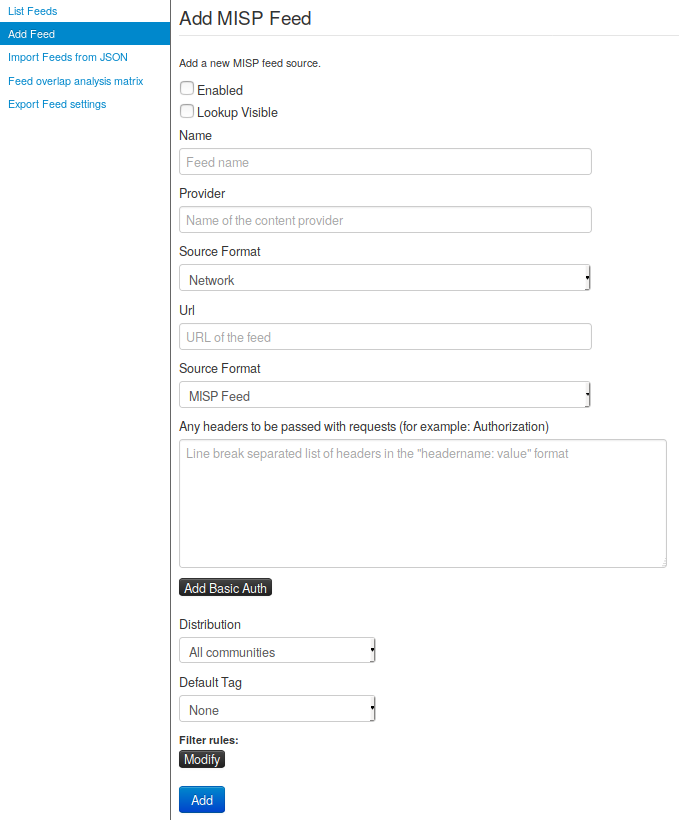
\includegraphics[width=1.0\linewidth]{pics/feeds3.png}
        \end{minipage}
        \hfill
        \begin{minipage}{0.48\linewidth}
            \begin{itemize}
                \item Enabled
                \item Lookup visible
                \item Name
                \item Provider
                \item Source Format
                \item Url
                \item Source Format
                \item Headers
                \item Distribution
                \item Default Tag
                \item Filter rules
            \end{itemize}
        \end{minipage}
\end{frame}

\begin{frame}[t,fragile] {Q\&A}

\includegraphics[scale=0.5]{misplogo.pdf}
\begin{itemize}
        \item \url{https://github.com/MISP/PyMISP}
        \item \url{https://github.com/MISP/}
        \item We welcome new functionalities and pull requests.
\end{itemize}

\end{frame}

